\documentclass{standalone}
\usepackage{tikz}
\usepackage{xcolor}
\usetikzlibrary{patterns, positioning}
\usetikzlibrary{shapes.misc}
\usepackage[outline]{contour}
\contourlength{1.5pt} 


\begin{document}
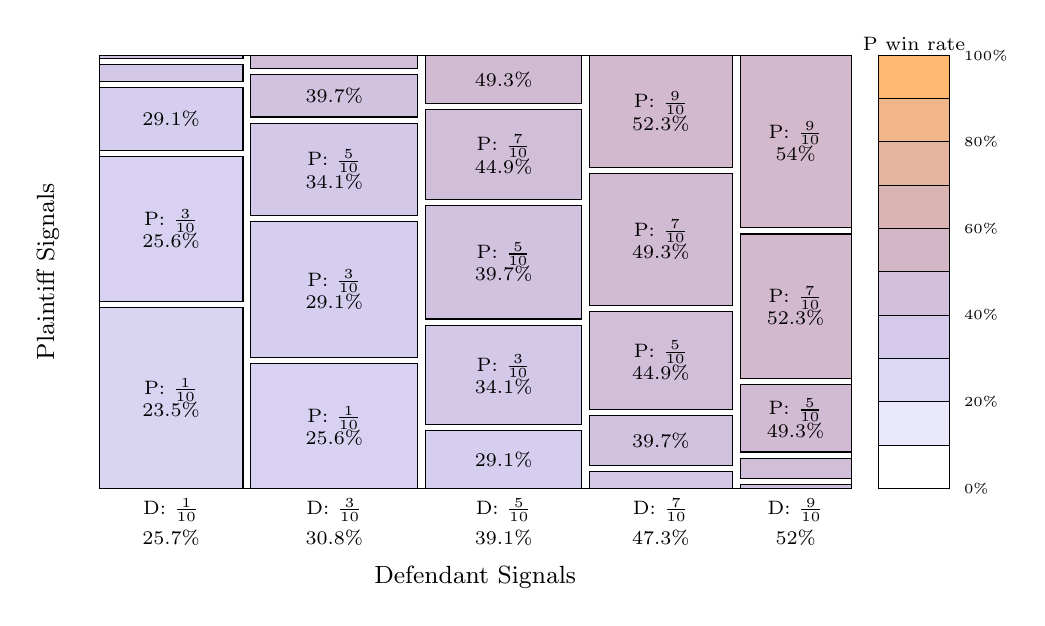
\begin{tikzpicture}
\newcommand{\DFractionOffset}{0.4}
\newcommand{\AxisLabelYAdjust}{-0.235}
\draw[draw=black] (0.6,2) rectangle (10.15,7.5);
\draw[fill=blue!76!orange!24!white!80!white, draw=black] (0.6,2) rectangle (2.4266,4.2939);
\draw (1.5133055457271263, 3.1469416538511563) node[font=\scriptsize, text=black, align=center] {P: $\frac{1}{10}$\\ 23.5\%};
\draw[fill=blue!74!orange!26!white!80!white, draw=black] (0.6,4.3739) rectangle (2.4266,6.2094);
\draw (1.5133055457271263, 5.291654611906873) node[font=\scriptsize, text=black, align=center] {P: $\frac{3}{10}$\\ 25.6\%};
\draw[fill=blue!71!orange!29!white!78!white, draw=black] (0.6,6.2894) rectangle (2.4266,7.0864);
\draw (1.5133055457271263, 6.687929768558263) node[font=\scriptsize, text=black, align=center] {29.1\%};
\draw[fill=blue!66!orange!34!white!77!white, draw=black] (0.6,7.1664) rectangle (2.4266,7.3812);
\draw[fill=blue!60!orange!40!white!75!white, draw=black] (0.6,7.4612) rectangle (2.4266,7.5);
\draw (1.5133055457271263, 1.6) node[anchor=north, font=\scriptsize, text=black] {25.7\%};
\draw (1.5133055457271263, {1.6 + \DFractionOffset}) node[anchor=north, font=\scriptsize, text=black] {D: $\frac{1}{10}$};
\draw[fill=blue!74!orange!26!white!80!white, draw=black] (2.5266,2) rectangle (4.648,3.5805);
\draw (3.5873182448342513, 2.79023283586639) node[font=\scriptsize, text=black, align=center] {P: $\frac{1}{10}$\\ 25.6\%};
\draw[fill=blue!71!orange!29!white!78!white, draw=black] (2.5266,3.6605) rectangle (4.648,5.3859);
\draw (3.5873182448342513, 4.523194470279333) node[font=\scriptsize, text=black, align=center] {P: $\frac{3}{10}$\\ 29.1\%};
\draw[fill=blue!66!orange!34!white!77!white, draw=black] (2.5266,5.4659) rectangle (4.648,6.6372);
\draw (3.5873182448342513, 6.051550063389358) node[font=\scriptsize, text=black, align=center] {P: $\frac{5}{10}$\\ 34.1\%};
\draw[fill=blue!60!orange!40!white!75!white, draw=black] (2.5266,6.7172) rectangle (4.648,7.2524);
\draw (3.5873182448342513, 6.984788255366081) node[font=\scriptsize, text=black, align=center] {39.7\%};
\draw[fill=blue!55!orange!45!white!73!white, draw=black] (2.5266,7.3324) rectangle (4.648,7.5);
\draw (3.5873182448342513, 1.6) node[anchor=north, font=\scriptsize, text=black] {30.8\%};
\draw (3.5873182448342513, {1.6 + \DFractionOffset}) node[anchor=north, font=\scriptsize, text=black] {D: $\frac{3}{10}$};
\draw[fill=blue!71!orange!29!white!78!white, draw=black] (4.748,2) rectangle (6.7273,2.7355);
\draw (5.737674834900076, 2.3677623256697258) node[font=\scriptsize, text=black, align=center] {29.1\%};
\draw[fill=blue!66!orange!34!white!77!white, draw=black] (4.748,2.8155) rectangle (6.7273,4.0709);
\draw (5.737674834900076, 3.4431999747193123) node[font=\scriptsize, text=black, align=center] {P: $\frac{3}{10}$\\ 34.1\%};
\draw[fill=blue!60!orange!40!white!75!white, draw=black] (4.748,4.1509) rectangle (6.7273,5.5936);
\draw (5.737674834900076, 4.872218198061088) node[font=\scriptsize, text=black, align=center] {P: $\frac{5}{10}$\\ 39.7\%};
\draw[fill=blue!55!orange!45!white!73!white, draw=black] (4.748,5.6736) rectangle (6.7273,6.8114);
\draw (5.737674834900076, 6.242501893005347) node[font=\scriptsize, text=black, align=center] {P: $\frac{7}{10}$\\ 44.9\%};
\draw[fill=blue!51!orange!49!white!72!white, draw=black] (4.748,6.8914) rectangle (6.7273,7.5);
\draw (5.737674834900076, 7.195721343993846) node[font=\scriptsize, text=black, align=center] {49.3\%};
\draw (5.737674834900076, 1.6) node[anchor=north, font=\scriptsize, text=black] {39.1\%};
\draw (5.737674834900076, {1.6 + \DFractionOffset}) node[anchor=north, font=\scriptsize, text=black] {D: $\frac{5}{10}$};
\draw[fill=blue!66!orange!34!white!77!white, draw=black] (6.8273,2) rectangle (8.6405,2.2163);
\draw[fill=blue!60!orange!40!white!75!white, draw=black] (6.8273,2.2963) rectangle (8.6405,2.9225);
\draw (7.733915368509571, 2.60942188431232) node[font=\scriptsize, text=black, align=center] {39.7\%};
\draw[fill=blue!55!orange!45!white!73!white, draw=black] (6.8273,3.0025) rectangle (8.6405,4.2447);
\draw (7.733915368509571, 3.623590842840515) node[font=\scriptsize, text=black, align=center] {P: $\frac{5}{10}$\\ 44.9\%};
\draw[fill=blue!51!orange!49!white!72!white, draw=black] (6.8273,4.3247) rectangle (8.6405,5.9949);
\draw (7.733915368509571, 5.1597967970394505) node[font=\scriptsize, text=black, align=center] {P: $\frac{7}{10}$\\ 49.3\%};
\draw[fill=blue!48!orange!52!white!71!white, draw=black] (6.8273,6.0749) rectangle (8.6405,7.5);
\draw (7.733915368509571, 6.787468910005718) node[font=\scriptsize, text=black, align=center] {P: $\frac{9}{10}$\\ 52.3\%};
\draw (7.733915368509571, 1.6) node[anchor=north, font=\scriptsize, text=black] {47.3\%};
\draw (7.733915368509571, {1.6 + \DFractionOffset}) node[anchor=north, font=\scriptsize, text=black] {D: $\frac{7}{10}$};
\draw[fill=blue!60!orange!40!white!75!white, draw=black] (8.7405,2) rectangle (10.15,2.0503);
\draw[fill=blue!55!orange!45!white!73!white, draw=black] (8.7405,2.1303) rectangle (10.15,2.3826);
\draw[fill=blue!51!orange!49!white!72!white, draw=black] (8.7405,2.4626) rectangle (10.15,3.3172);
\draw (9.44525323271662, 2.889873265790036) node[font=\scriptsize, text=black, align=center] {P: $\frac{5}{10}$\\ 49.3\%};
\draw[fill=blue!48!orange!52!white!71!white, draw=black] (8.7405,3.3972) rectangle (10.15,5.2304);
\draw (9.44525323271662, 4.313765266363499) node[font=\scriptsize, text=black, align=center] {P: $\frac{7}{10}$\\ 52.3\%};
\draw[fill=blue!46!orange!54!white!70!white, draw=black] (8.7405,5.3104) rectangle (10.15,7.5);
\draw (9.44525323271662, 6.40518508482704) node[font=\scriptsize, text=black, align=center] {P: $\frac{9}{10}$\\ 54\%};
\draw (9.44525323271662, 1.6) node[anchor=north, font=\scriptsize, text=black] {52\%};
\draw (9.44525323271662, {1.6 + \DFractionOffset}) node[anchor=north, font=\scriptsize, text=black] {D: $\frac{9}{10}$};
\node[font=\small, text=black] at (5.375, {1.1 + \AxisLabelYAdjust}) {Defendant Signals};
\node[font=\small, text=black, rotate=90] at (-0.050000000000000044, 4.75) {Plaintiff Signals};
\draw[draw=black] (10.5,2) rectangle (11.4,7.5);
\draw (10.95, 7.65) node[font=\scriptsize, text=black] {P win rate};
\draw[fill=blue!100!orange!0!white!88!white, draw=black] (10.5,2) rectangle (11.4,2.55);
\draw[fill=blue!89!orange!11!white!84!white, draw=black] (10.5,2.55) rectangle (11.4,3.1);
\draw[fill=blue!78!orange!22!white!81!white, draw=black] (10.5,3.1) rectangle (11.4,3.65);
\draw[fill=blue!67!orange!33!white!77!white, draw=black] (10.5,3.65) rectangle (11.4,4.2);
\draw[fill=blue!56!orange!44!white!73!white, draw=black] (10.5,4.2) rectangle (11.4,4.75);
\draw[fill=blue!44!orange!56!white!70!white, draw=black] (10.5,4.75) rectangle (11.4,5.3);
\draw[fill=blue!33!orange!67!white!66!white, draw=black] (10.5,5.3) rectangle (11.4,5.85);
\draw[fill=blue!22!orange!78!white!62!white, draw=black] (10.5,5.85) rectangle (11.4,6.4);
\draw[fill=blue!11!orange!89!white!59!white, draw=black] (10.5,6.4) rectangle (11.4,6.95);
\draw[fill=blue!0!orange!100!white!55!white, draw=black] (10.5,6.95) rectangle (11.4,7.5);
\draw (11.46, 2) node[anchor=west, font=\tiny, text=black] {0\%};
\draw (11.46, 3.1) node[anchor=west, font=\tiny, text=black] {20\%};
\draw (11.46, 4.2) node[anchor=west, font=\tiny, text=black] {40\%};
\draw (11.46, 5.3) node[anchor=west, font=\tiny, text=black] {60\%};
\draw (11.46, 6.4) node[anchor=west, font=\tiny, text=black] {80\%};
\draw (11.46, 7.5) node[anchor=west, font=\tiny, text=black] {100\%};


\end{tikzpicture}
\end{document}